\graphicspath{{./assets/}}
\setcounter{mtc}{1}
\chapter{Generalized context of the project }
\fancyhead[R]{\ungaramond\small\textbf{Chapter I. Generalized context of the project}}
\minitoc
\newpage
\section{The project's background}
\subsection{Overview on the host organization  }

\subsubsection{Company Background }
Systnaps is a technology company based in Paris, France that specializes in providing innovative software solutions to businesses across various industries. It prides itself with the expertise in areas such as data analytics, artificial intelligence, machine learning, and cloud computing. The following figure illustrates the company logo: 

\begin{figure}[!ht]\centering

\includegraphics[width=0.5\textwidth,angle=00]{assets/fa.png}
\caption{Systnaps Logo}
\end{figure}

Huxium, an affiliate of Systnaps is a technology company that specializes in providing customized software solutions to businesses across various industries. 


\begin{figure}[!ht]\centering

\includegraphics[width=0.5\textwidth,angle=00]{assets/fb.png}
\caption{Huxium Logo}
\end{figure}


 \subsubsection{Mission and Vision }

Systnaps was founded with the mission of helping businesses harness the power of technology to improve their operations, enhance customer experiences, and drive growth. They offer a range of services to meet the diverse needs of their clients, including custom software development, application maintenance and IT consulting. 

\subsubsection{Core Services or Products }

The core services of Systnaps in the data management space include: 
\begin{itemize}[label={--}]
    \item Database Management: Securely managing databases for businesses, including tasks such as administration, optimization, and recovery. 

\item Data Integration: Assisting businesses in integrating and managing data across multiple systems and platforms, encompassing activities like migration, warehousing, and synchronization. 

\item Big Data: Supporting businesses in managing and analyzing large volumes of data (often known as "big data"), involving tasks such as processing, visualization, and machine learning. 

\item  Data Governance: Helping businesses ensure compliance with regulatory and legal requirements in managing their data, encompassing activities such as privacy and security, classification, and retention. 

 \end{itemize}

\subsubsection{Market Position and notable clients }

While they do not have a significant global presence, they have established themselves as a reputable player in the French IT market. 

Systnaps has worked with clients across a range of industries, including finance, healthcare, and media. The following figure showcases some of the current clients: 


\begin{figure}[!ht]\centering

\includegraphics[width=0.8\textwidth,angle=00]{assets/fc.png}
\caption{Company clients}
\end{figure}


\subsection{Project description }

Our end-of-studies project entails designing and implementing a comprehensive Platform as a Service (PaaS) solution on the cloud. This PaaS platform incorporates various networking, storage, and automation services.

Specifically, the project focuses on designing and implementing networking services such as load balancing, ingress, and authentication/authorization. These services are crucial for managing traffic flow and ensuring secure access to the platform.

Additionally, the project involves implementing a distributed and redundant storage backend that encompasses both object and block storage. This ensures reliable and scalable storage capabilities.

Furthermore, highly available and replicated database storage services are integrated into the PaaS platform to ensure consistent and dependable data access for users.

The project also encompasses utility services such as a private registry for storing artifacts and automated CI/CD operations to streamline the deployment process.

Lastly, the PaaS platform incorporates a robust and efficient disaster recovery strategy to quickly recover from any unplanned downtime or service interruptions.

In summary, this end-of-studies project demonstrates a comprehensive understanding of cloud computing and DevSecOps principles. It showcases the ability to design and implement a comprehensive PaaS platform with essential services to support modern application development and deployment. 

\subsection{Analysis of existing processes }

The current infrastructure relies on a few monolithic virtual private servers and utilizes Docker Compose for container orchestration. Within this infrastructure, there are multiple Docker Compose stacks serving different purposes, including: 
\begin{itemize}[label={--}]
\item An application development stack: This stack houses essential applications for software development, such as code editors, compilers, and development frameworks. 

\item A utility stack : includes a self-hosted enterprise instance of GitLab, which serves as a version control system and facilitates continuous integration and continuous deployment (CI/CD) processes for applications. Additionally, the stack includes a self-hosted instance of Nextcloud, a file hosting and sharing platform utilized for storing and sharing files relevant to application development. 

\item A reverse proxy stack: This stack comprises three Docker images - acme-companion, docker-gen, and nginx - functioning as a reverse proxy for the application. Nginx acts as the web server, routing traffic to the application, while acme-companion and docker-gen generate SSL/TLS certificates and automatically update the Nginx configuration. 
\end{itemize}

While Docker Compose provides a lightweight and scalable infrastructure for application development, the reliance on monolithic virtual private servers can hinder scalability and infrastructure maintenance. Consolidating all services on a single server creates a single point of failure and increases the risk of downtime. 

\subsection{Constructive criticism on existing processes} 

Based on cloud computing and DevOps best practices, the following is some of the weak points of such an infrastructure :

\begin{itemize}[label={--}]

\item Docker Compose for orchestration: While suitable for small-scale projects, it becomes challenging to manage and maintain as the number of services and containers grows. Kubernetes offers a more scalable and efficient solution for container orchestration and management. 

\item Lack of a distributed storage backend: The absence of distributed storage can lead to data loss or inconsistency during node failures. Kubernetes provides built-in options like persistent volumes, stateful sets, and storage classes for distributed storage. 

\item Absence of an authorization and authentication backend: The lack of an authorization and authentication system can result in security vulnerabilities and unauthorized access to sensitive data. Kubernetes offers several options for authentication and authorization, including role-based access control (RBAC), webhook token authentication, and client certificate authentication. 

\item Missing disaster recovery strategy: Without a disaster recovery plan, there is a risk of significant downtime and data loss during unforeseen events. Kubernetes provides options for disaster recovery, such as backup and restore mechanisms, failover and recovery strategies, and multi-zone deployments. 

\item Use of large and inefficient container images: Large and inefficient container images can lead to slower deployment times, increased storage requirements, and decreased performance. DevOps best practices, coupled with Kubernetes features like image caching, rolling updates, and horizontal scaling, can optimize container image management and deployment. 

\end{itemize}

In conclusion, adopting Kubernetes and implementing cloud computing and DevOps best practices can significantly enhance the scalability, reliability, security, and performance of the IT ecosystem. 

\subsection{Problem statement }

In today's fast-paced business environment, the company is looking to leverage cloud computing and DevSecOps practices to gain a competitive edge.  

However, building and managing a PaaS platform that provides reliable and scalable infrastructure services is a complex and challenging task. The lack of a well-designed and integrated PaaS platform can lead to increased costs, inefficient resource utilization, and security vulnerabilities. 

The objective of this project is to design, build and implement a PaaS platform that provides a complete set of infrastructure services, including networking, storage, database, and utility services, along with a resilient and efficient disaster recovery strategy. The platform will also incorporate DevSecOps practices to ensure security and compliance with industry standards. 

The main challenge of this project is to ensure the scalability, availability, and security of the PaaS platform while providing a simple and intuitive user experience for developers. This requires a deep understanding of cloud computing and DevSecOps practices, along with expertise in networking, storage, database, and utility services. 

The successful implementation of this project will enable the company to accelerate their digital transformation journey, reduce operational costs, and improve their overall business agility. 

 

\subsection{Ideation and proposed solutions} 

The company has decided to explore the possibility of moving to a cloud-based infrastructure to increase scalability, availability, and security. After analyzing various options, we have decided to propose a self-managed PaaS platform based on Kubernetes that contains the following components: 

\begin{itemize}[label={--}]

\item Networking services: The networking services will be provided by MetalLB for layer 4 load balancing, Traefik as an ingress controller, and Cert-manager for TLS provisioning. The platform will also use Authelia, OpenLDAP, and Redis for authentication/authorization. 

\item A Storage backend: The storage backend will be provided by Ceph, which is a distributed and redundant storage backend for both object and block storage. This will ensure that data is highly available and can be easily scaled. 

\item Highly available and replicated database storage services: The platform will use both MongoDB and PostgreSQL as highly available and replicated database storage services for both the relational and document models. This will provide the necessary data persistence and redundancy required for a PaaS platform. 

\item DevSecOPS utility services: The platform will use several utility services to help store artifacts, automate CI/CD operations, and improve code quality. These services include Jenkins as the CI/CD orchestrator, ArgoCD as the CD controller, SonarQube for code scanning, Harbor as a private registry, and Jenkins pipelines to automate building applications, scanning, and delivery. 

\item Disaster recovery strategy: The platform will have a resilient and efficient disaster recovery strategy that uses Velero to back up Kubernetes related objects and proprietary Python programs to backup database data. This will ensure that the platform is highly available, even in the event of a disaster. 

\end{itemize}

Overall, the proposed solution will provide a highly available, scalable, and secure PaaS platform that can meet the company's needs for application development and deployment. The platform will also have a robust disaster recovery strategy, which will ensure business continuity in the event of an outage.  


\newpage  % if no new page table will not be in the good place
\section{Project planning}
\subsection{Project management }
\subsubsection{Comparative research }

\begin{table}[h!]
\center
\begin{tabular}[b]{|m{3cm}|m{4cm}|m{4cm}|m{4cm}|}
\hline
\rowcolor{white}
 & Waterfall (V model) 
 & Agile   & DevOPS  \\
\hline
 Lifecycle  
& Linear software development approach 
& Incremental and iterative sprint cycles. 
& Uses automation techniques to enable continuous deployment of change. \\
\hline
 Automation level  
& Low 
& Varied 
& High 
 \\
\hline
 Delivery of value 
& Slow (Scale : months) 
& Rapid (daily/weekly) 
& Continuous  \\
\hline
 Responsiveness to business needs 
& Extremely limited 
& Responsive 
& Highly responsive   \\
\hline
 Collaboration 
& Low: teams operate in functional silos 
& Improved: short dev cycles 
& High: cross-functional teams are involved from project start. \\
\hline
Quality 
& Low: issues are only identified after tests 
& Improved: issues are identified after every sprint 
& High: Unit testing and code quality checks are performed during development. \\
\hline
 Risk 
& Increases as project development progresses 
& Decreases as project development progresses 
& Decreases as project development progresses \\
\hline
\end{tabular}
\caption{ comparative study}
\textcolor{white}{I} \label{tab:tab-m}
\end{table}

Based on the previous comparative study, it is apparent that the approach most suited to our use case is one that helps improve collaboration, reduce context-switching, introduce automation, and enable observability and monitoring. 

\subsubsection{Agile devSecOPS }

When evaluating devSecOPS as a practice and Agile as a delivery approach, it is important to note that they are not mutually exclusive. In spite of the evident differences between DevSecOPS and the Agile methodology, their overall goal of increasing speed and delivering quality software is similar in nature and together they produce great products and improve the software development.

\begin{figure}[!ht]\centering
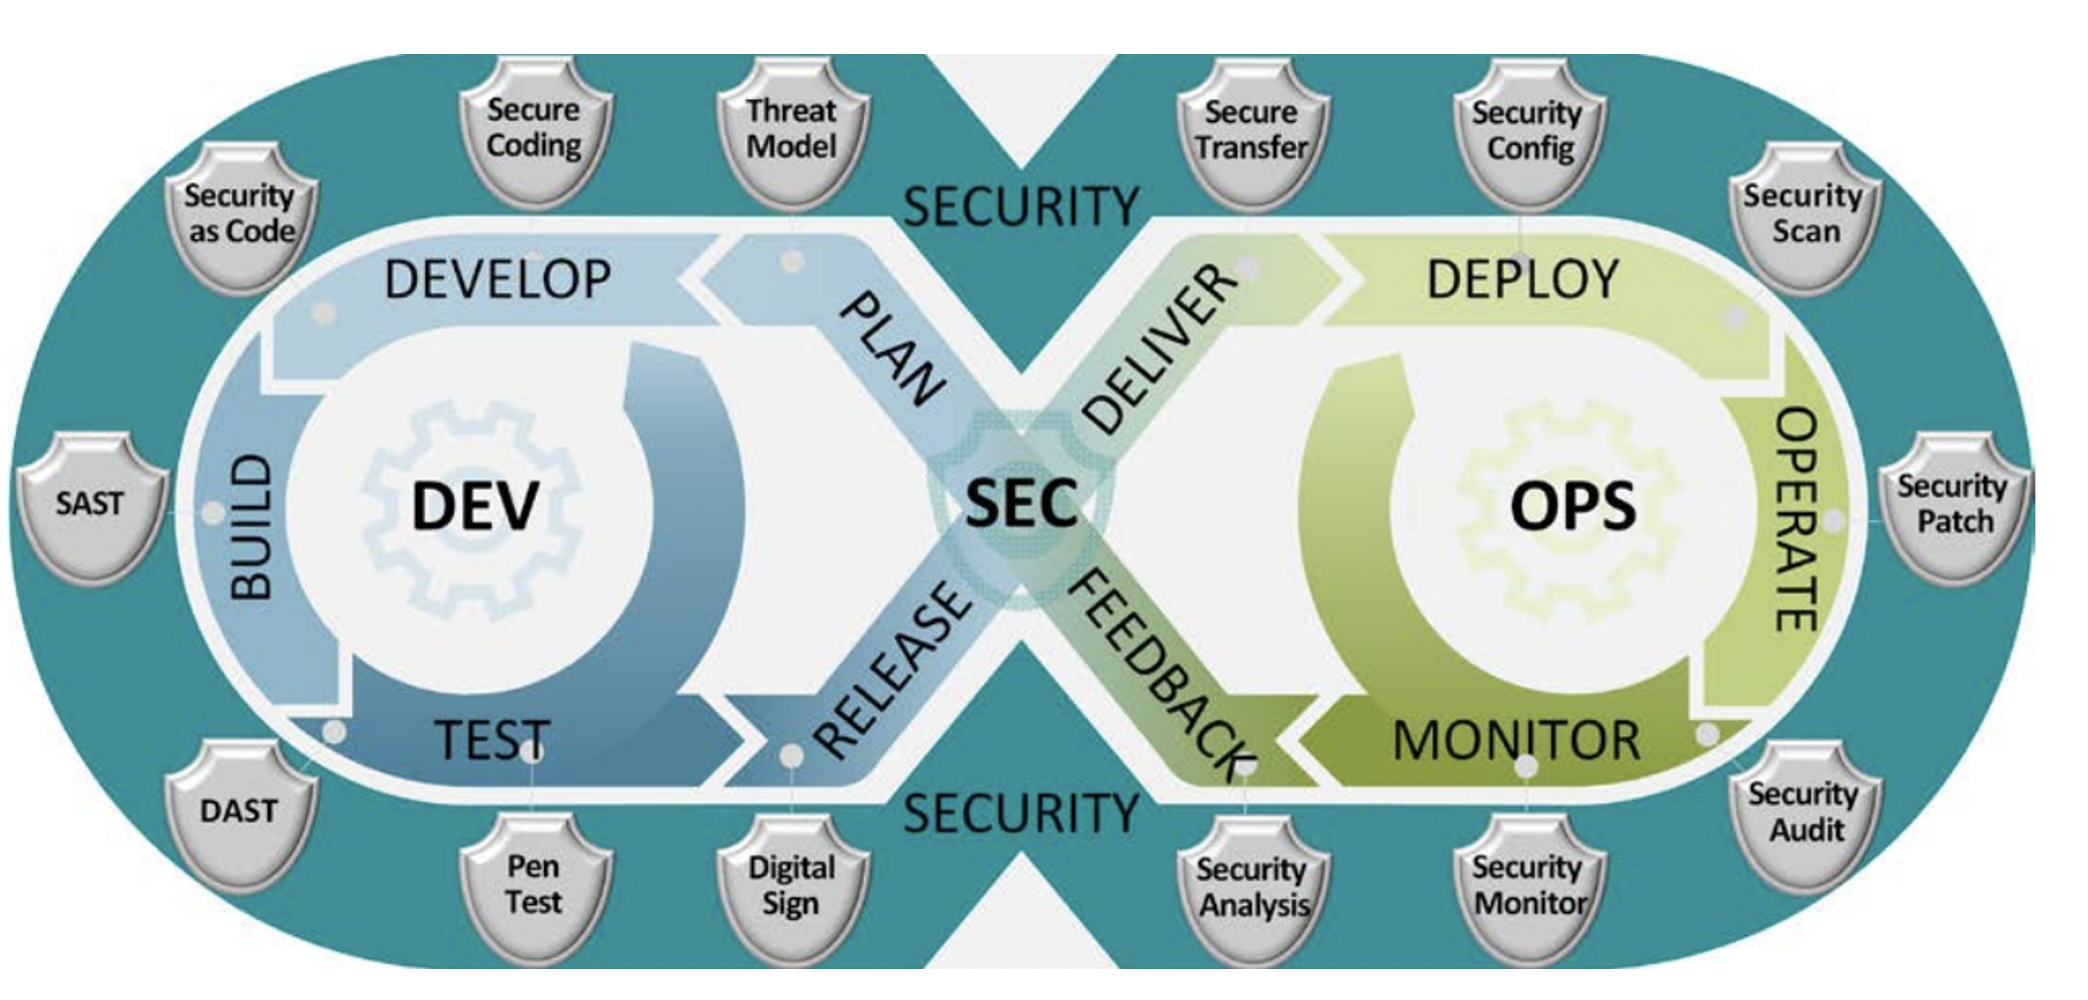
\includegraphics[width=0.8\textwidth,angle=00]{assets/f1.png}
\caption{Process overview}
\label{fig:processOverview}
\end{figure}

The following figure showcases an overview of the process and the key DevSecOPS roles. 
\paragraph{DevSecOPS Evangelist:} 
Usually the DevSecOPS team leader, he focuses on promoting the DevSecOPS advantages, identifying and quantifying companies’ benefits deriving from a higher agility. 

\paragraph{Release Manager:} 
The product stability manager which is basically the product owner. He cares about the product’s management and coordination. 

\paragraph{Automation Architect: }
Provides a complete automation role involving the DevSecOPS and Cloud solutions. He is an integration specialist that ensures the high availability of the pre-production and production systems. 

\paragraph{Software Developer/Tester:}
DevSecOPS developers are not responsible only for the transformation of new requirements into code, they also have to deal with testing, distribution and continuous monitoring processes.

\paragraph{Security Engineer: }
The DevSecOPS approach implements security by design.

\newpage 

\subsection{Capturing requirements}
Our analysis is aimed at identifying the key actors in our design, the functional and non-functional needs our system is to provide for.

\subsubsection{Identifying key actors}
In this context, an actor is a user or any other system that interacts with the subject by exchanging signals and data.

\paragraph{Cloud architecture related actors:}
In order to have a devSecOPS compliant approach, it needs to be built on top of a containerized, highly available cloud infrastructure:
\begin{itemize}[label={--}]
\item Cloud architect: He is responsible for designing and implementing cloud computing solutions.
\item IaC tools: Although being a piece of software, it is necessary in order to automate provisioning and configuration of resources.
\item Cloud provider: Usually a third-party entity that allows for elastically allocating resources.
\item DevSecOPS team: A devSecOPS engineer is the consumer in this case, he uses the provisioned resources to build an ecosystem that is compliant with organizational needs.
\end{itemize}

\paragraph{CI/CD related actors:}
The cloud resources hold the value of a tool that is then leveraged to assist the development process:
\begin{itemize}[label={--}]
\item DevSecOPS team: uses the provisioned resources and follows an agile devSecOPS approach to build an ecosystem that is compliant with organizational needs.
\item Developer: A consumer of the devSecOPS ecosystem as well as the CI/CD workflow.
\item Company client: He is the end user and provides the specifications on software development.
\end{itemize}

\subsubsection{Functional requirements}

Formulating an understanding on functional requirements is a primordial phase in the implementation of the subject.

\begin{itemize}[label={--}]
\item A cloud-based infrastructure capable of hosting the devSecOPS ecosystem in terms of compute resources, storage and networking.
\item A continuous integration platform : The desired goal is to provide a CI workflow that channels the development effort in order to continuously ensure code quality.
\item A CD workflow: provide an automated and continuous delivery and deployment process.
\end{itemize}

\subsubsection{Non-functional requirements}

\begin{itemize}[label={--}]
\item High availability and resilience: Typically satisfied by distributed backend resources, orchestration and load balancing of workloads. 
\item Performance and scalability: Usually dependent on the cloud provider as well as the used technologies.
\item Security: An inbuilt quality that cloud and DevSecOPS offer by design.
\item Observability: A highly achievable need due the pluggability of containerized environments.
\item Usability: A somewhat hard to achieve requirement due to the rarity of a technologically adept workforce. 
\item Relatively low cost : the need to prioritize self-hosting and adopting opensource alternatives.
\end{itemize}

\newpage
\subsection{Product backlog }

\subsubsection{Backlog history }
\begin{longtable}[H]{|m{1cm}|m{3cm}|m{1cm}|m{7cm}|m{1.2cm}|}
\hline
 {\textbf{Epic ID}} & {\textbf{EPIC}} & {\textbf{Story ID}} & {\textbf{Story}} & {\textbf{Prior-ity}} \\
 \hline
\endhead
0 & \raggedright Certified devSecOps training &	0.1 &	Managing and running custom VMs. & \\
\cline{3-5}
&   & 0.2 &	Managing docker containers.	& \\
\cline{3-5}
&   & 0.3 &	CI/CD pipelines. & \\
\hline
1 & Maintenance and cleanup. &	1.1	& Exploring existing infrastructure and resources. & \\
\cline{3-5}
&   &	1.2 & Performing maintenance on enterprise assets. & \\

\hline
2 & Cloud design &	2.1 &	Information gathering phase. & \\
\hline
3 & Resource provisioning &	3.1 &	Provisioning resources using IaC playbooks. & \\
\hline
4 & Infrastructure setup. &	4.1 &	Infrastructure setup using IaC playbooks. & \\
\hline
5 & \raggedright Initial PaaS setup. &	5.1 &	Setting up ingress controller and TLS certificate provisioner.	 & \\
\cline{3-5}
&   & 5.2 &	Setting distributed storage backend.	 & \\
\cline{3-5}
&   & 5.3 &	Setting up network load balancer.	 & \\
  \hline
6 & Deployment of CI/CD platform &	6.1 &	Setting up personalized CI/CD orchestrator.	 & \\
\cline{3-5}
&   & 6.2 &	Setting up quality gate (CI).	 & \\
\cline{3-5}
&   & 6.3 & Setting up CD controller.	 & \\
  \hline
7 & \raggedright Preparation of automated CICD workflows. &	7.2 &	Structuring SCM backend	 & \\

\cline{3-5}
&   & 7.2 &	 \raggedright Using GitOPS and devOPS tools to automate CI/CD pipelines.	 & \\
\hline
\pagebreak
\hline
8 & \raggedright Deployment of authentication / authorization backend 	& 8.1 & \raggedright Self-managing distributed database storage backends (redis, mongoDB, postgresql).	 & \\
\cline{3-5}
&   & 8.2 &	\raggedright Deployment and configuration of authentication and authorization services.	 & \\
\cline{3-5}
&   & 8.3 &	\raggedright Configuring forward auth middlewares for secure access.	 & \\
   \hline
9 & \raggedright Implement a resilient disaster recovery strategy. & 9.1 &\raggedright  Provisioning cloud storage resources.		 & \\
\cline{3-5}
&   & 9.2 & \raggedright Preparing and applying backup strategy for application specific data.	 & \\
\cline{3-5}
&   & 9.3 &	\raggedright Preparing and applying backup strategy for PaaS specific workloads.	 & \\
 \hline
\caption{ Backlog History Table }
\end{longtable}
% \raggedright for space issue


\newpage
\subsubsection{Sprint planning }
The project lasted seven months and a half starting on March 1st 2022. Overall, ten sprints have been followed with the typical duration of 3 weeks for each. 


\begin{longtable}[H]{|m{2cm}|m{10cm}|m{2cm}|}
\hline
 {\textbf{Sprint ID}} & {\textbf{Sprint Details }} & {\textbf{Duration }} \\ \hline 
0 
&
The first period was spent following a company sponsored devSecOps training. The following elements have been covered: 
Creating vm images using packer, spinning up virtual machines using vagrant,  
Using docker, docker compose plugin and docker container orchestration in swarm, 
An overview on CI/CD pipelines using Jenkins. 
&
4 weeks  \\
\hline
1 
&
The following three weeks were dedicated to exploring the existing infrastructure. Performing some maintenance and planning for migration. 
&
3 weeks  \\ \hline
2 
&
Next, we have started the information gathering phase in which we have formed an initial overview of the desired goals we would like to reach. 
&
2 weeks \\ \hline
3 
&
The use of IaC allowed us to provision the main cloud resources dedicated to hosting the PaaS infrastructure. 
&
2 weeks \\ \hline
4 
&
An initial setup of the provisioned resources was then automated and performed. 
&
3 weeks \\ \hline
5 
&
Putting in place the basic PaaS services, namely a distributed storage backend, a layer 2 load balancer, a cloud-native layer 4 ingress controller to route requests serving also as a reverse proxy and an application load balancer. 
&
3 weeks \\ \hline
6 
&
Mounting the backing CI/CD services which are mostly personalized to company needs. 
&
3 weeks \\ \hline
7 
&
Levering the CI/CD ecosystem to put in place pipelines to automate product testing, code quality checks, and delivery. 
&
4 weeks \\ \hline
8 
&
Securing access to company assets using an Authentication/Authorization middleware. 
&
3 weeks \\ \hline
9 
&
Putting in place a disaster recovery strategy that leverages distributed storage and S3 compliant object storage. 
&
3 weeks \\ \hline

\caption{ Sprint planning}
\end{longtable}

\newpage

\subsection{Technological choices }
% \paragraph{Development tools }
In this section, we layout the cloud provider choice,
\subsubsection{Cloud provider choice: } 

\paragraph{OVH\cite{OVHcloud}: }

A decisive factor concerning the cloud provider choice is related to company’s desire to opt mainly for a provider that is based in France.  

\paragraph{Openstack\cite{OpenStack}: }

OVH uses openstack as its backing cloud computing infrastructure. Thus, conversing with components as neutron, nova, glance, swift is a must. 

\subsubsection{Infrastructure as code tools }

\paragraph{Terraform\cite{Terraform}: }

An industry standard for conversing with cloud providers in order to provision and configure resources. 

\paragraph{Ansible\cite{Ansible}: }

We have opted for ansible because it’s faster than its alternatives namely chef, and easier to use.  

\subsubsection{Containerization and orchestration techniques: }

\paragraph{Container orchestrator: Kubernetes v1.21\cite{Kubernetes} }

An open source container orchestration tool that automates the deployment, scaling, and managing containerized applications. 

\paragraph{Container runtime : containerd }

A daemon for linux that manages the complete container lifecycle. 

\paragraph{Container platform : docker-ce v20.10 }

The container management tool that uses containerd to manage container lifecycles and their underlying abstractions such as volumes and networking.  

\paragraph{Container networking: Calico }

A cloud-native plugin deployment in Kubernetes that uses the CNI API to provide a networking and security solution in the cluster. 

\paragraph{Container platform : docker-ce v20.10 }

The container management tool that uses containerd to manage container lifecycles and their underlying abstractions such as volumes and networking. 

\paragraph{Container networking: Calico }

A cloud-native plugin deployment in Kubernetes that uses the CNI API to provide a networking and security solution in the cluster. 


\subsubsection{Self-hosted PaaS services }

\paragraph{Distributed storage backend: Ceph\cite{Ceph} }

A highly reliable, open source, distributed storage platform offering bloc , filesystem and object storage volumes to be leveraged by the orchestrator. 

\paragraph{Ingress Controller: Traefik ingress controller }

An open-source edge router serving as an ingress controller, a reverse proxy and a load balancer. 

\paragraph{Layer 2 load balancer: MetalLB}

This opensource load balancer provides support for bare metal Kubernetes clusters using standard protocols. 

\paragraph{Private registry: harbor }

An open-source private registry serving as a backend to sore artifacts in a secure manner. 

\paragraph{Database storage (document): Redis, MongoDB }

Database storage in document format is provided by a replicated mongoDB cluster. An in memory redis cluster allows for session storage. 

\paragraph{Database storage (SQL): PostgreSQL }

A PostgreSQL cluster in HA mode coupled with a PGpool middleware to distribute load and control replication. 

\paragraph{Authentication middleware: Authelia }

An open-source portal serving as an authentication and authorization server. It leverages the “forward auth” capability of the ingress controller to regulate access. 

\paragraph{User management: OpenLDAP }

An open-source implementation of the Lightweight Directory Access Protocol that is used to manage organizational user credentials and details. 

\paragraph{SCM tool: Gitlab }

An enterprise solution for source code management and versioning. 

\paragraph{CI/CD orchestration: Jenkins }

An open-source automation server which enables build, test, and deployment processes. 

\paragraph{Quality gate: SonarQube }

An open-source platform that allows for continuous inspection of code quality. 

\paragraph{CD controller: ArgoCD, ArgoRollouts }

An open-source declarative, GitOPS continuous delivery tool for Kubernetes. 

\paragraph{Disaster recovery: Velero }

An open-source tool to safely backup and restore, perform disaster recovery, and migrate Kubernetes cluster resources and persistent volumes. 

\paragraph{Config formats: YAML, TOML, HCP config, JSON }

\subsubsection{Development tools }

\paragraph{Development IDE: VS Code }

A pluggable, lightweight opensource IDE. 

\paragraph{SSH platform: Termius }

A platform that offers port forwarding and secure file transfer over ssh. 

\subsubsection{Development languages }

\paragraph{Scripting: python\cite{Python}, shell, groovy\cite{Groovy} }

Shell was used to interface with the linux operating system. For conversing with APIs, an assortment of python scripts were developed to automate various tasks, namely, database backups. Jenkins pipelines and configurations were written in groovy. 

\paragraph{Templating: YTT\cite{YTT}, jinja2\cite{Jinja2} }

To template various configuration files that are dependent on the deployment environment, we used YTT for YAML/JSON. Jinja2 was the main templating tool for ansible playbooks. 

\newpage

\subsection{Architectural specifications}

\subsubsection{Physical architecture}

The following figure is an overview of the infrastructure resource setup. It is to be discussed in further detail in the following chapters:

\begin{figure}[H]\centering
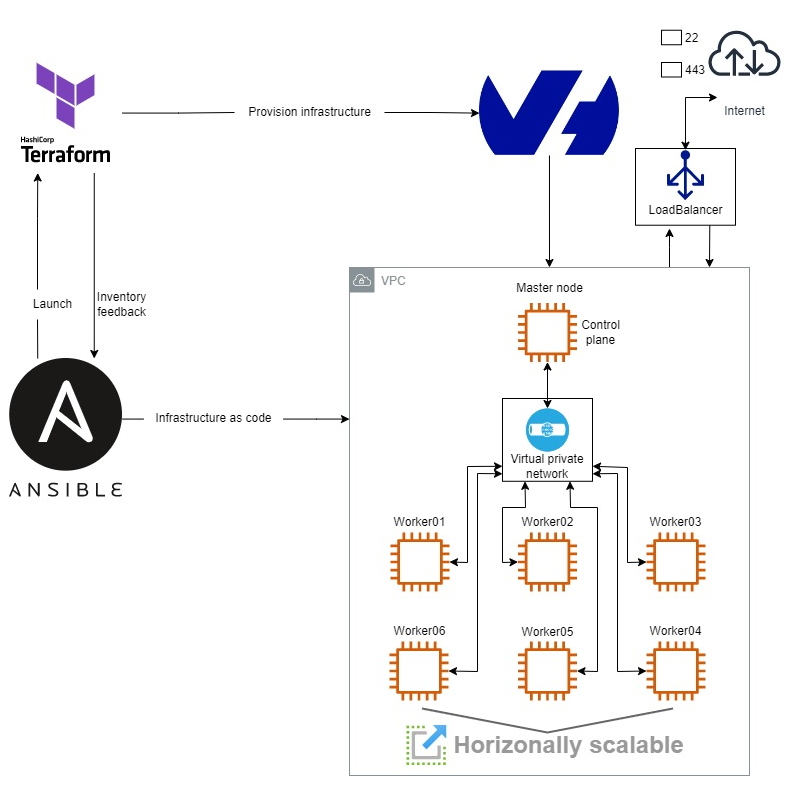
\includegraphics[width=1.0\textwidth,angle=00]{assets/f7.jpg}
\caption{Physical architecture}
\label{fig:f7}
\end{figure}

\newpage

\subsubsection{PaaS deployment architecture} 
Next we layout the organization of the subsystems, software classes, and layers that make the complete logical system of our PaaS infrastructure :

\begin{figure}[H]\centering
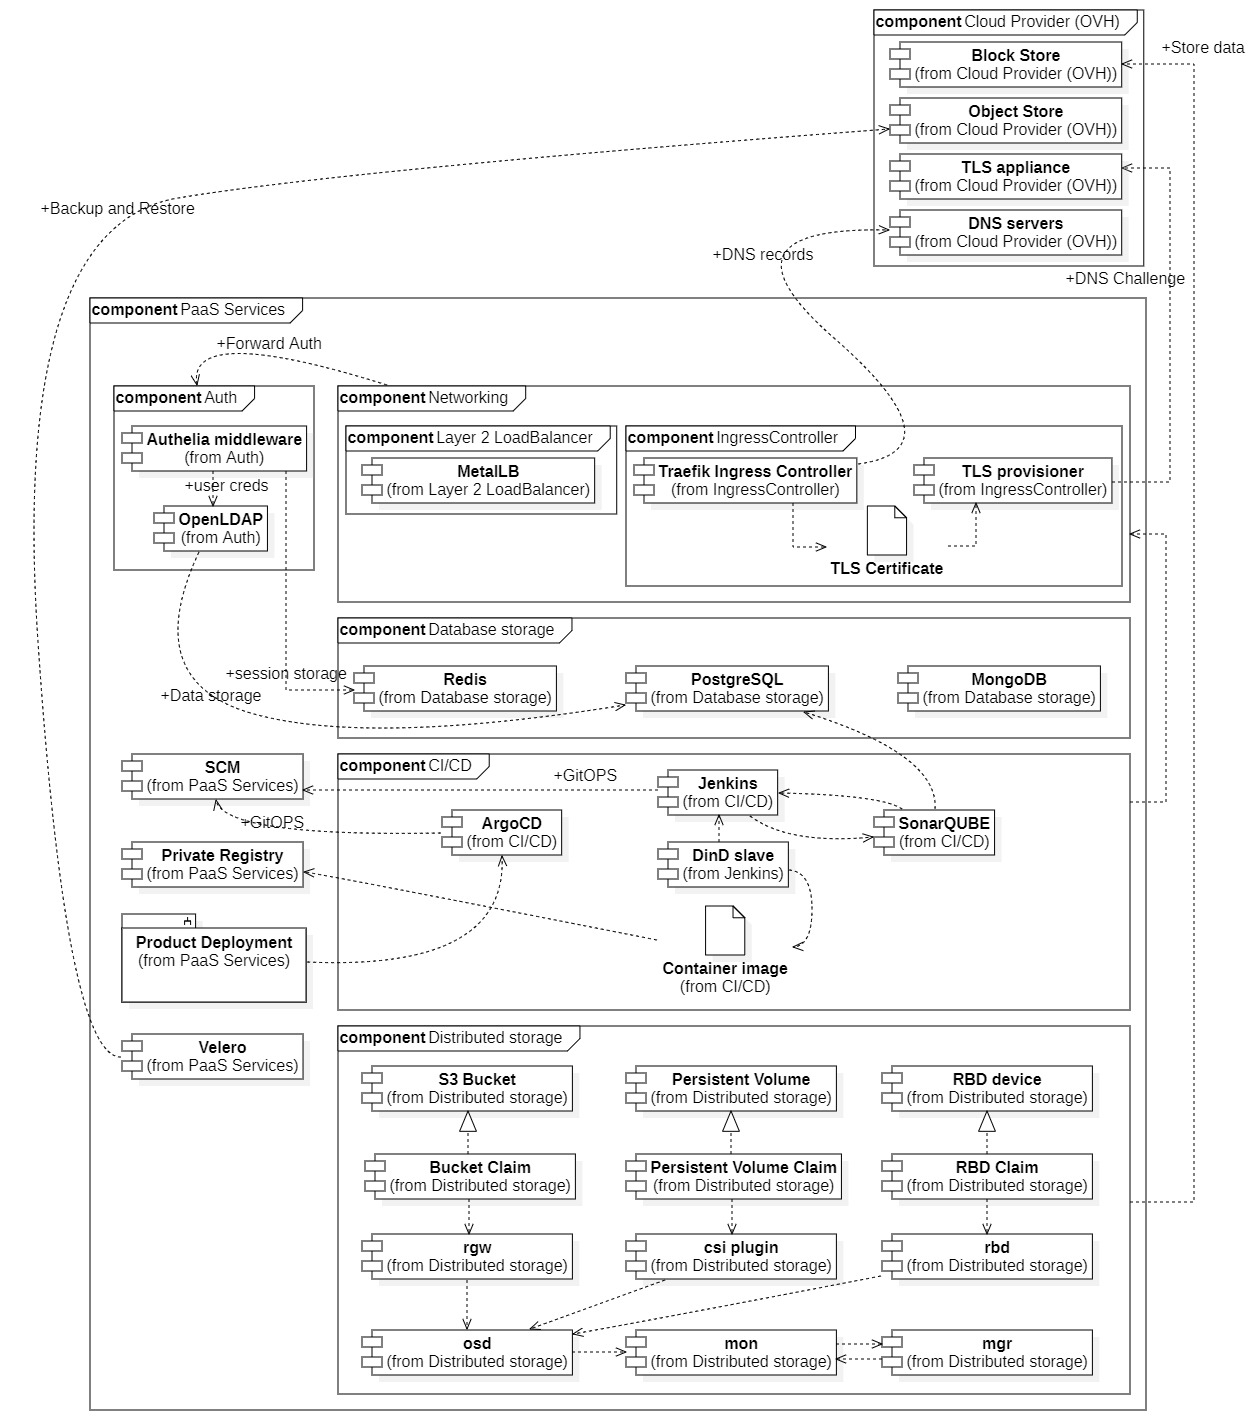
\includegraphics[width=1.0\textwidth,angle=00]{assets/f8.jpg}
\caption{PaaS infrastructure}
\label{fig:f8}
\end{figure}

\newpage

\subsection{Workspace description}

To implement the project, the company has provided us with the necessary hardware equipment, certified preliminary training as well as the desired cloud resources. This allowed us to engage in real-world projects, collaborate with experienced professionals, and expand our skills.

\section*{Conclusion}
In conclusion, requirement analysis is a crucial step in any project, especially when it comes to cloud computing and DevOps.  

By identifying and understanding the requirements of the project, we have created a solid foundation that ensures the success of the implementation phase. 

The requirement analysis process has involved identifying the project goals, defining the user personas, and outlining the technical requirements of the project. It has also involved determining the specific business requirements, infrastructure requirements, and application requirements. 

All of these requirements are critical to ensuring that the PaaS environment is tailored to meet the specific needs of the organization. 

By conducting a thorough requirement analysis, ensured that the project is well-defined, properly scoped, and that the stakeholders' expectations are appropriately managed. It provides a solid framework for making informed decisions about the design and implementation of the PaaS environment, as well as determining the tools and technologies that will be used.